
\begin{frame}[noframenumbering]{}
\end{frame}

\begin{frame}[noframenumbering]{Imperfections -- Chutes de tension ohmiques}
    \begin{columns}
        \begin{column}{0.5\linewidth}
            \centering
            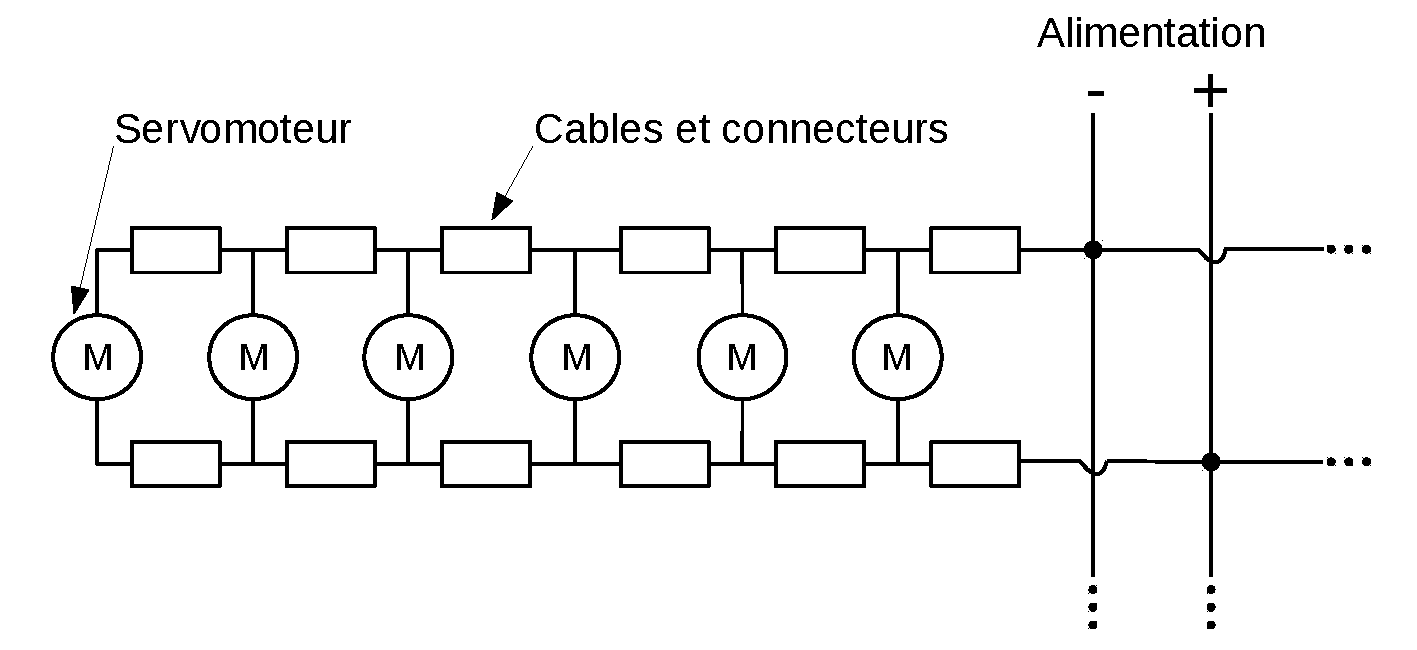
\includegraphics[type=pdf,ext=.pdf,read=.pdf,width=1.0\linewidth]{../schema/electric_bus}
        \end{column}
        \begin{column}{0.5\linewidth}
            \centering
            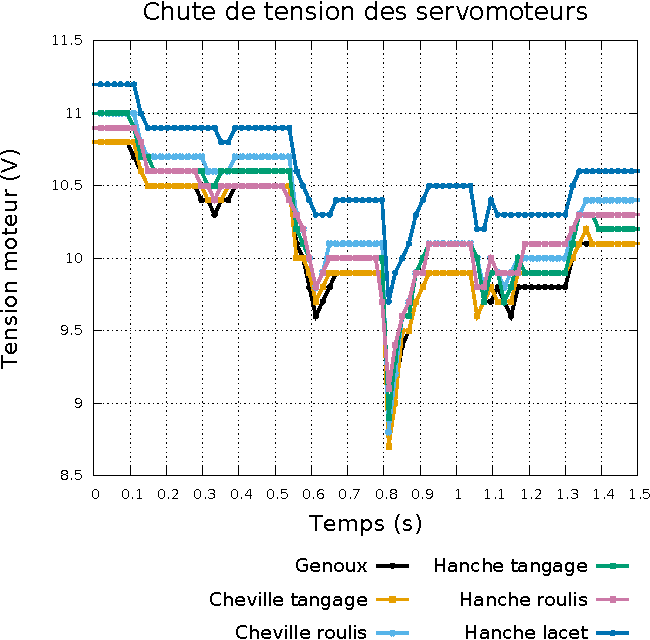
\includegraphics[type=pdf,ext=.pdf,read=.pdf,width=1.0\linewidth]{../plot/motors_voltage}
        \end{column}
    \end{columns}
    \begin{itemize}
        \item Usure des connecteurs $\Rightarrow$ résistance électrique
        \item Chutes de la tension sur le bus
        \item $\Rightarrow$ Affaiblissement du couple maximum
    \end{itemize}
\end{frame}


\begin{frame}[noframenumbering]{Mouvement de marche}
    \begin{columns}
        \begin{column}{0.4\textwidth}
            \begin{itemize}
                \item Générateur \textit{IKWalk} boucle ouverte + stabilisation
                \item Holonome
                \item Réglage manuel par expérimentation
                \item Mouvement désiré $\neq$ mesuré
                \item Amélioration 2017 : générateur \textit{QuinticWalk}
            \end{itemize}
        \end{column}
        \begin{column}{0.6\textwidth}
            \centering
            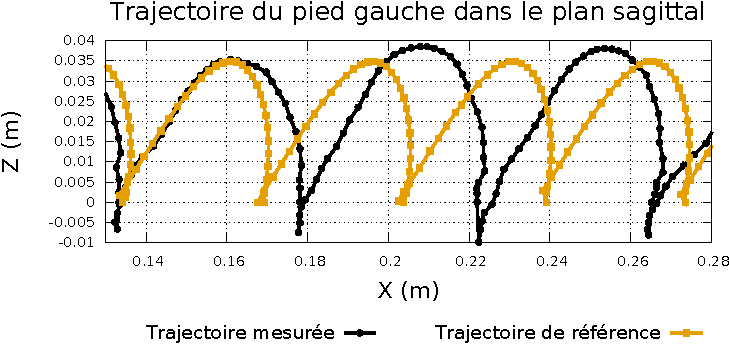
\includegraphics[type=pdf,ext=.pdf,read=.pdf,width=1.0\linewidth]{../plot/walk_traj_foot}
        \end{column}
    \end{columns}
    \vspace{0.2cm}
    \begin{block}{}
        \customtextcolor{
            \small
            \textit{Rhoban hardware and software open source contributions for robocup humanoids}}\\
        \scriptsize
        Quentin Rouxel, Grégoire Passault, Ludovic Hofer, Steve N'Guyen, Olivier Ly\\
        Workshop on Humanoid Soccer Robots, 2015\\
    \end{block}
\end{frame}

\begin{frame}[noframenumbering]{Mouvement de marche (2/3) -- Générateur \textit{IKWalk}}
    \centering
    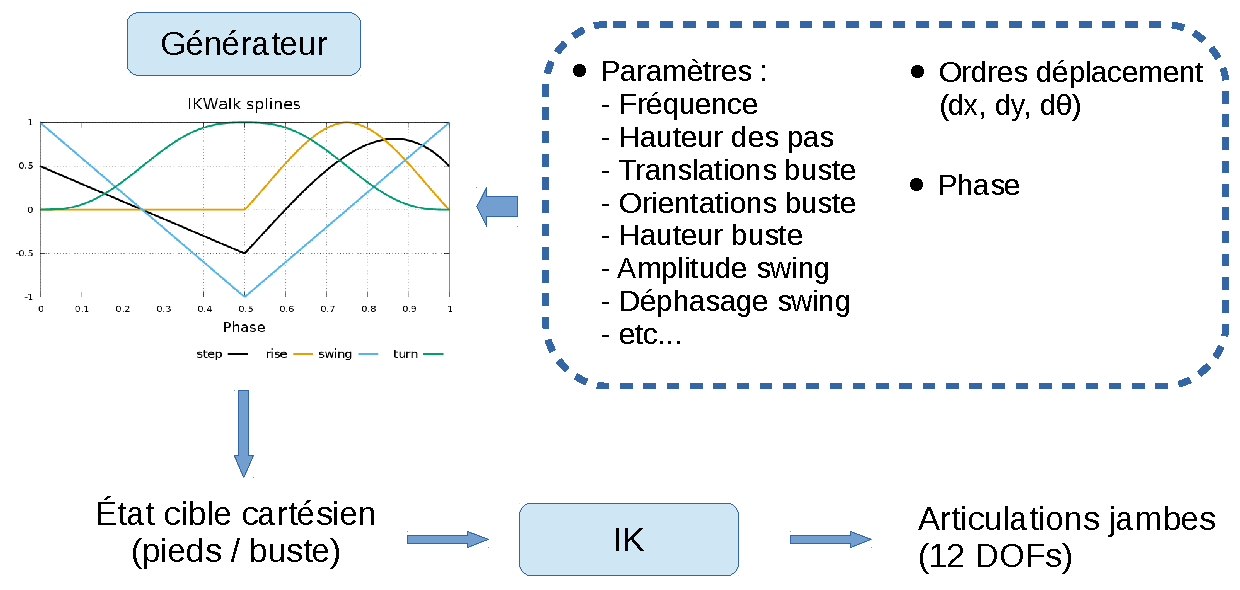
\includegraphics[type=pdf,ext=.pdf,read=.pdf,width=1.0\linewidth]{../schema/ikwalk}
    \begin{block}{}
        \customtextcolor{
            \small
            \textit{Rhoban hardware and software open source contributions for robocup humanoids}}\\
        \scriptsize
        Quentin Rouxel, Grégoire Passault, Ludovic Hofer, Steve N'Guyen, Olivier Ly\\
        Workshop on Humanoid Soccer Robots, 2015\\
    \end{block}
\end{frame}

\begin{frame}[noframenumbering]{Mouvement de marche (3/3) -- Stabilisation}
    \begin{columns}
        \begin{column}{0.5\textwidth}
            \begin{itemize}
                \item Stabilisation latérale
                \item Position du centre de pression
                \item Mise en pause du mouvement
            \end{itemize}
        \end{column}
        \begin{column}{0.5\textwidth}
            \centering
            \movie[
                autostart,
                width=\linewidth, 
                height=0.56\linewidth,
                poster,
                loop
            ]{}{../video/cutStabilization_light.mp4}
            \scriptsize
            (Source : Grégoire Passault)
        \end{column}
    \end{columns}
    \centering
    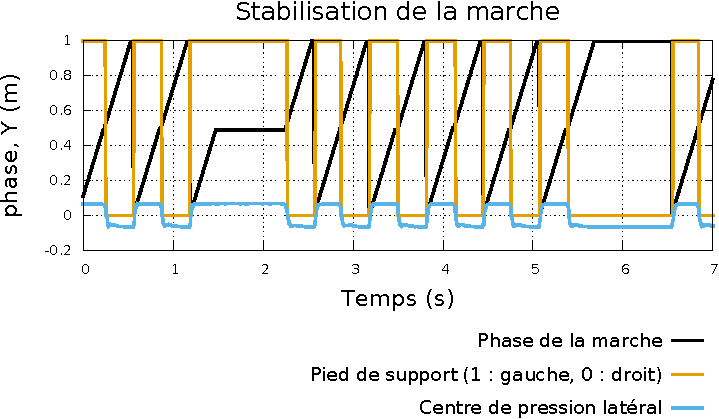
\includegraphics[type=pdf,ext=.pdf,read=.pdf,width=0.6\linewidth]{../plot/walk_stabilization1}
\end{frame}


\begin{frame}[noframenumbering]{QuinticWalk et ZMP}
    \centering
    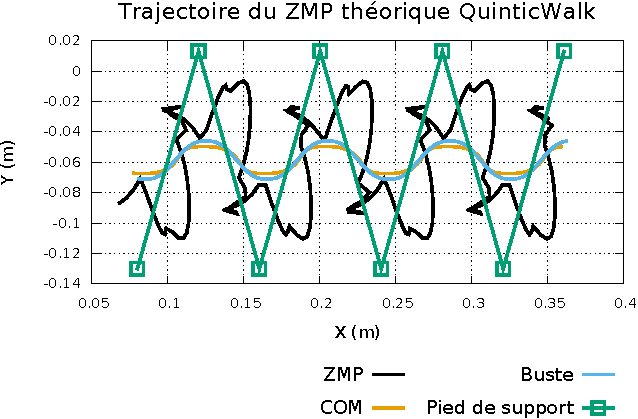
\includegraphics[type=pdf,ext=.pdf,read=.pdf,width=1.0\linewidth]{../plot/walk_quintic_zmp}
\end{frame}

\begin{frame}[noframenumbering]{Odométrie et LWPR -- LWPR}
    \centering
    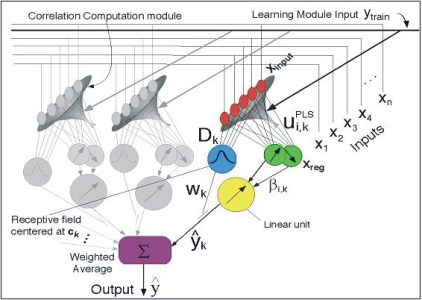
\includegraphics[width=0.6\linewidth]{../media/lwpr.jpg}\\
    \scriptsize
    (Source : Sethu Vijayakumar)
\end{frame}

\begin{frame}[noframenumbering]{Odométrie et LWPR}
    \centering
    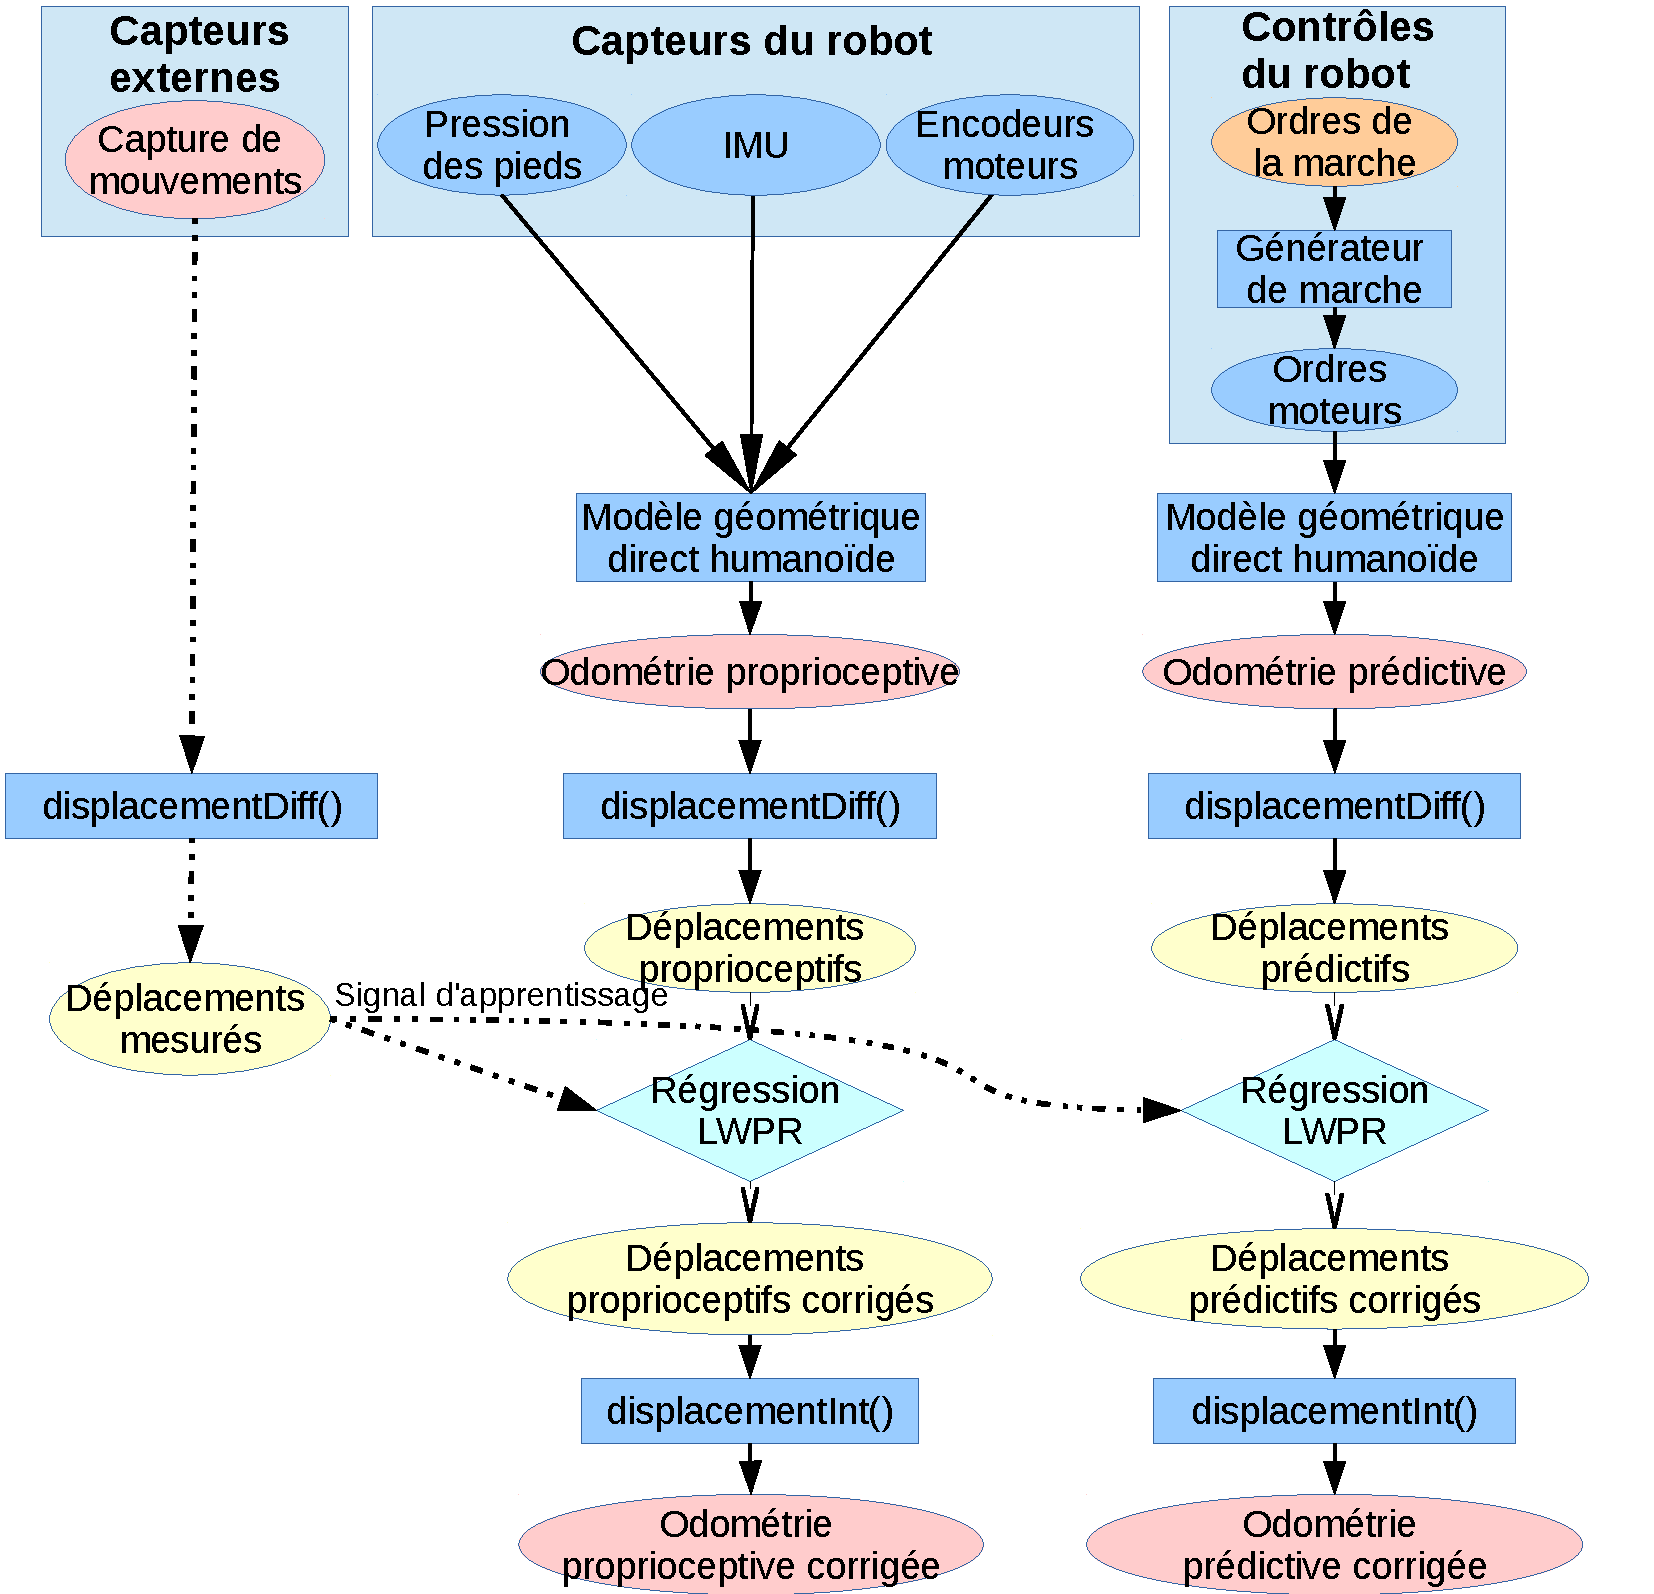
\includegraphics[type=pdf,ext=.pdf,read=.pdf,height=8.0cm]{../schema/architecture}
\end{frame}

\begin{frame}[noframenumbering]{Odométrie et LWPR -- Contextes}
    Contextes comparés :
    \begin{itemize}
        \item Surface de marche : 
            \begin{itemize}
                \item moquette
                \item herbe artificielle ($3$~cm)
            \end{itemize}
        \item Processus de stabilisation : 
            \begin{itemize}
                \item désactivé (boucle ouverte)
                \item activé (boucle fermée)
            \end{itemize}
    \end{itemize}
\end{frame}

\begin{frame}[noframenumbering]{Odométrie et LWPR -- Délai de l'IMU}
    \centering
    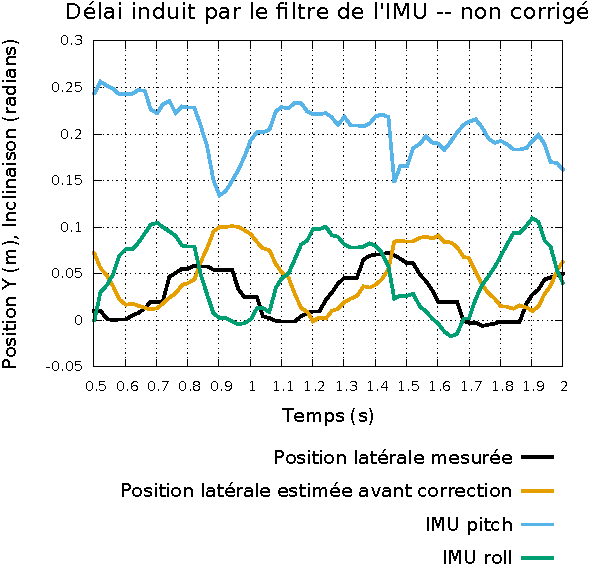
\includegraphics[type=pdf,ext=.pdf,read=.pdf,width=0.5\linewidth]{../plot/OdometryLWPR/grass_open_delay_imu_uncorrected}
    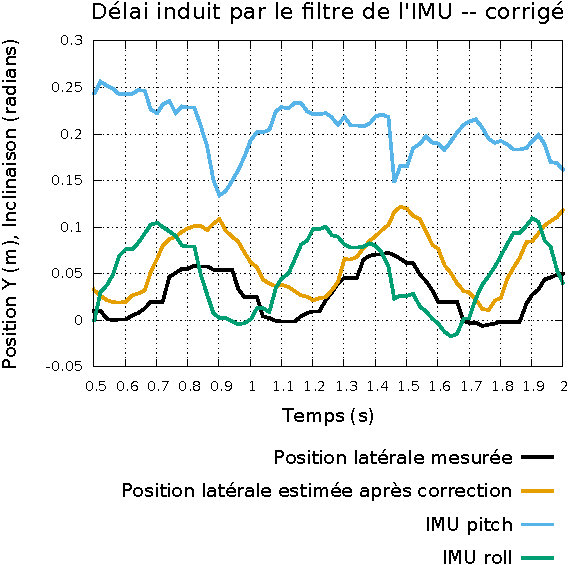
\includegraphics[type=pdf,ext=.pdf,read=.pdf,width=0.5\linewidth]{../plot/OdometryLWPR/grass_open_delay_imu_corrected}
\end{frame}

\begin{frame}[noframenumbering]{Odométrie et LWPR -- Données}
    \centering
    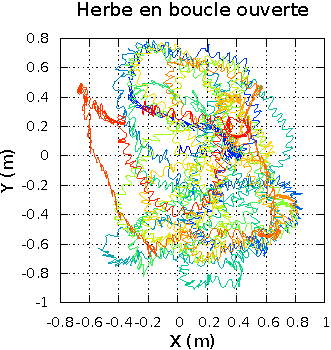
\includegraphics[type=pdf,ext=.pdf,read=.pdf,width=0.25\linewidth]{../plot/OdometryLWPR/grass_open_learn_log_complete_traj}
    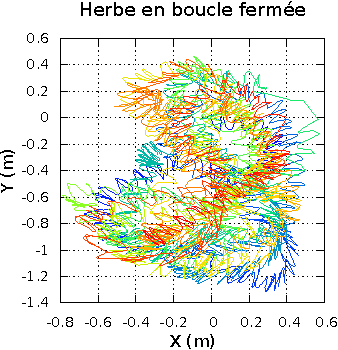
\includegraphics[type=pdf,ext=.pdf,read=.pdf,width=0.25\linewidth]{../plot/OdometryLWPR/grass_close_learn_log_complete_traj}
    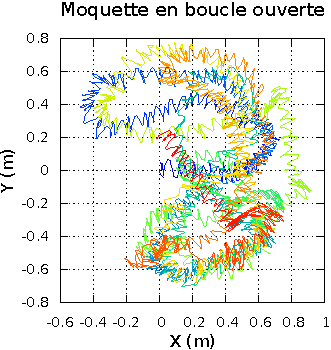
\includegraphics[type=pdf,ext=.pdf,read=.pdf,width=0.25\linewidth]{../plot/OdometryLWPR/carpet_open_learn_log_complete_traj}
    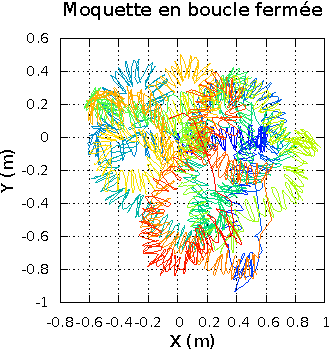
\includegraphics[type=pdf,ext=.pdf,read=.pdf,width=0.25\linewidth]{../plot/OdometryLWPR/carpet_close_learn_log_complete_traj}
    \newline
    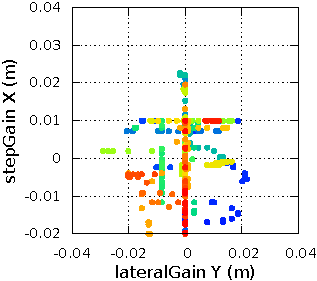
\includegraphics[type=pdf,ext=.pdf,read=.pdf,width=0.25\linewidth]{../plot/OdometryLWPR/grass_open_learn_log_walk_orders}
    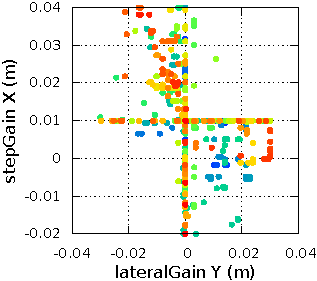
\includegraphics[type=pdf,ext=.pdf,read=.pdf,width=0.25\linewidth]{../plot/OdometryLWPR/grass_close_learn_log_walk_orders}
    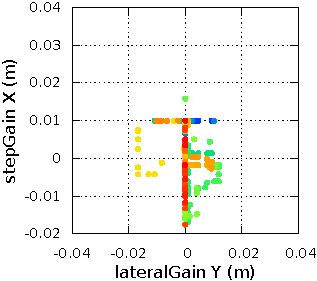
\includegraphics[type=pdf,ext=.pdf,read=.pdf,width=0.25\linewidth]{../plot/OdometryLWPR/carpet_open_learn_log_walk_orders}
    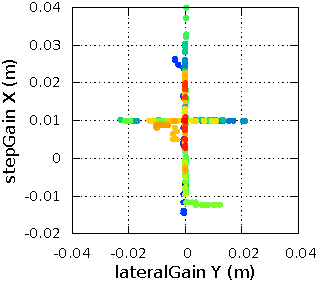
\includegraphics[type=pdf,ext=.pdf,read=.pdf,width=0.25\linewidth]{../plot/OdometryLWPR/carpet_close_learn_log_walk_orders}
    \newline
\end{frame}

\begin{frame}[noframenumbering]{Odométrie et LWPR -- Corrélations prédictives}
    \begin{columns}
        \begin{column}{0.35\linewidth}
            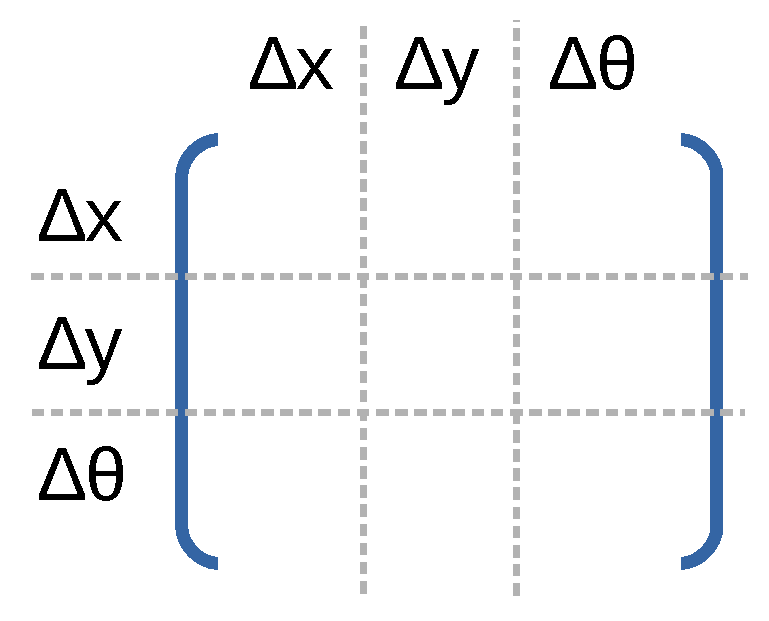
\includegraphics[type=pdf,ext=.pdf,read=.pdf,width=0.8\linewidth]{../schema/correlation_matrix}
        \end{column}
        \begin{column}{0.65\linewidth}
            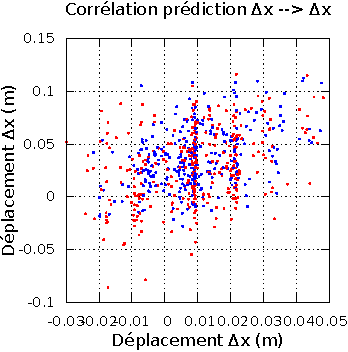
\includegraphics[type=pdf,ext=.pdf,read=.pdf,width=2.5cm]{../plot/OdometryLWPR/grass_close_function_goal_x_x}
            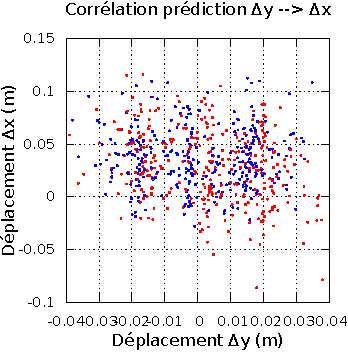
\includegraphics[type=pdf,ext=.pdf,read=.pdf,width=2.5cm]{../plot/OdometryLWPR/grass_close_function_goal_y_x}
            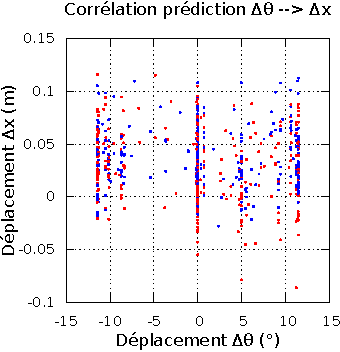
\includegraphics[type=pdf,ext=.pdf,read=.pdf,width=2.5cm]{../plot/OdometryLWPR/grass_close_function_goal_yaw_x}
            \vspace{0.2cm}
            \newline
            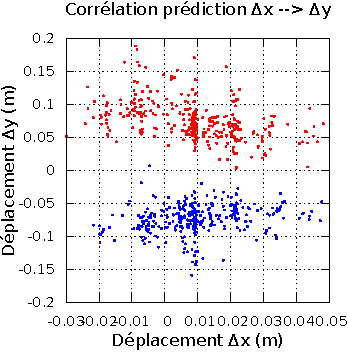
\includegraphics[type=pdf,ext=.pdf,read=.pdf,width=2.5cm]{../plot/OdometryLWPR/grass_close_function_goal_x_y}
            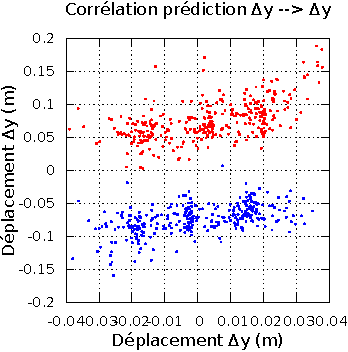
\includegraphics[type=pdf,ext=.pdf,read=.pdf,width=2.5cm]{../plot/OdometryLWPR/grass_close_function_goal_y_y}
            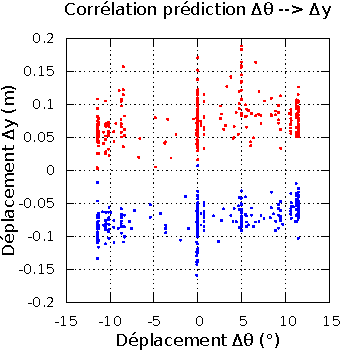
\includegraphics[type=pdf,ext=.pdf,read=.pdf,width=2.5cm]{../plot/OdometryLWPR/grass_close_function_goal_yaw_y}
            \vspace{0.2cm}
            \newline
            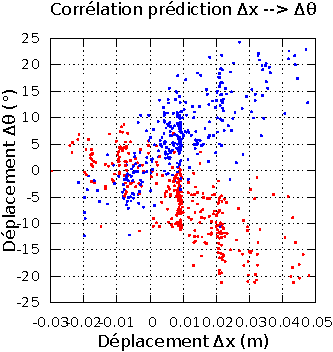
\includegraphics[type=pdf,ext=.pdf,read=.pdf,width=2.5cm]{../plot/OdometryLWPR/grass_close_function_goal_x_yaw}
            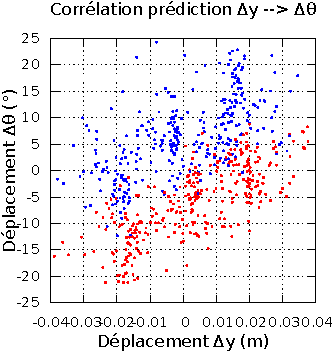
\includegraphics[type=pdf,ext=.pdf,read=.pdf,width=2.5cm]{../plot/OdometryLWPR/grass_close_function_goal_y_yaw}
            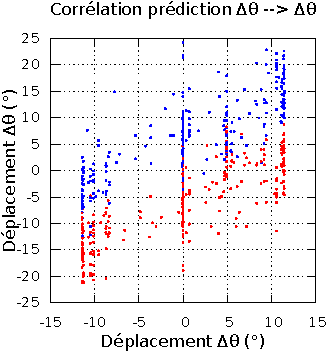
\includegraphics[type=pdf,ext=.pdf,read=.pdf,width=2.5cm]{../plot/OdometryLWPR/grass_close_function_goal_yaw_yaw}
        \end{column}
    \end{columns}
\end{frame}

\begin{frame}[noframenumbering]{Odométrie et LWPR -- Convergence}
    \centering
    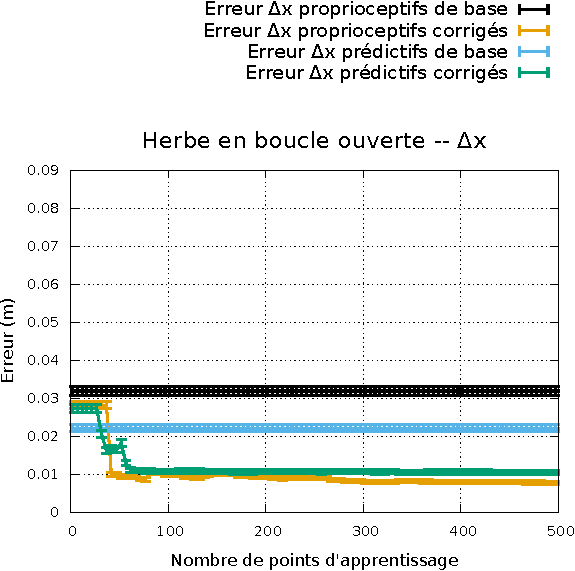
\includegraphics[type=pdf,ext=.pdf,read=.pdf,width=0.2\linewidth]{../plot/OdometryLWPR/grass_open_convergence_x}
    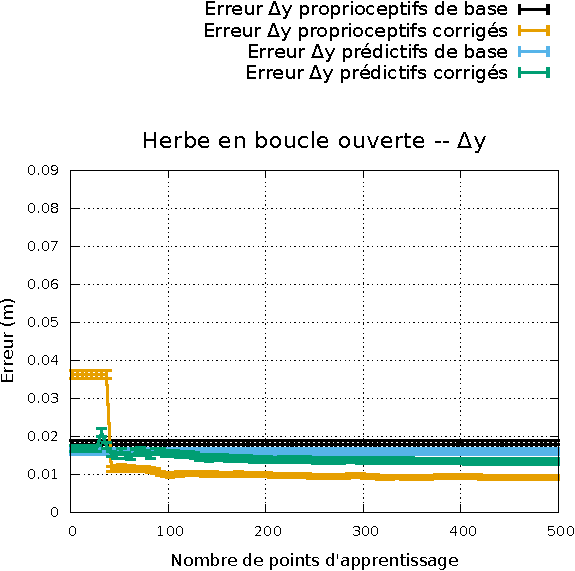
\includegraphics[type=pdf,ext=.pdf,read=.pdf,width=0.2\linewidth]{../plot/OdometryLWPR/grass_open_convergence_y}
    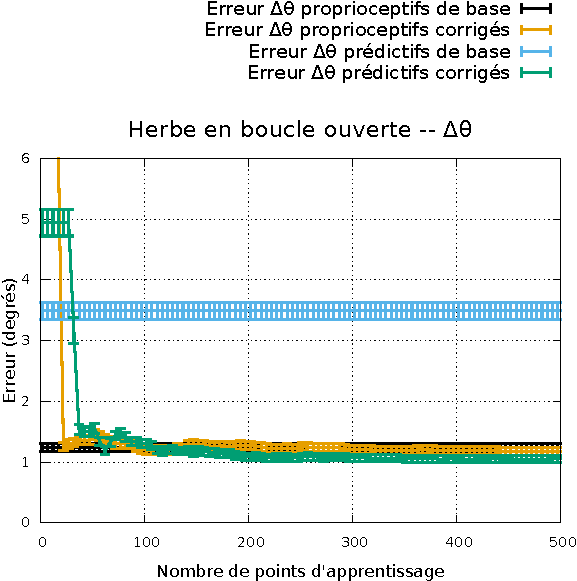
\includegraphics[type=pdf,ext=.pdf,read=.pdf,width=0.2\linewidth]{../plot/OdometryLWPR/grass_open_convergence_yaw}
    \newline
    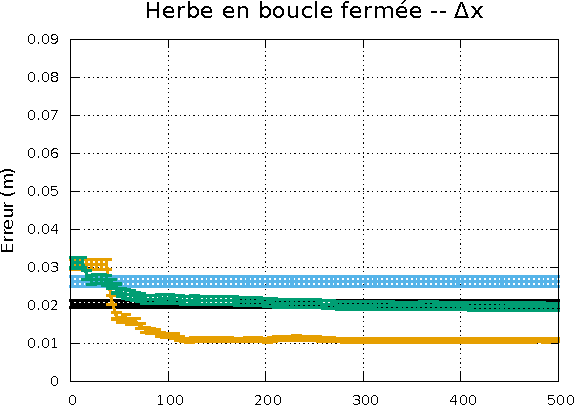
\includegraphics[type=pdf,ext=.pdf,read=.pdf,width=0.2\linewidth]{../plot/OdometryLWPR/grass_close_convergence_x}
    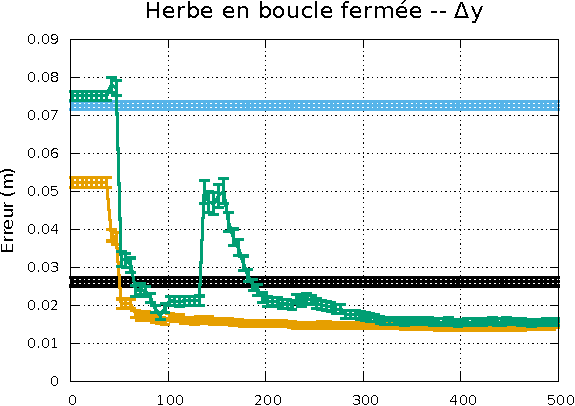
\includegraphics[type=pdf,ext=.pdf,read=.pdf,width=0.2\linewidth]{../plot/OdometryLWPR/grass_close_convergence_y}
    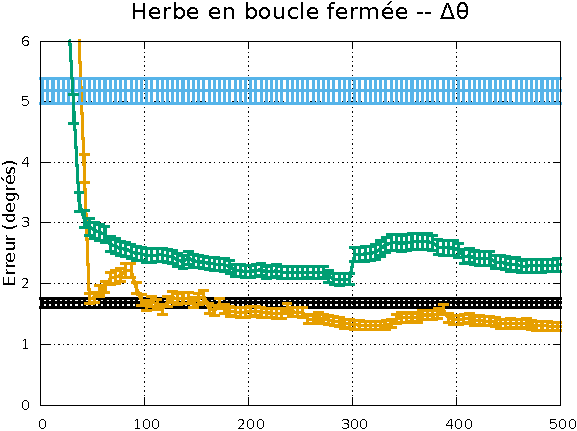
\includegraphics[type=pdf,ext=.pdf,read=.pdf,width=0.2\linewidth]{../plot/OdometryLWPR/grass_close_convergence_yaw}
    \newline
    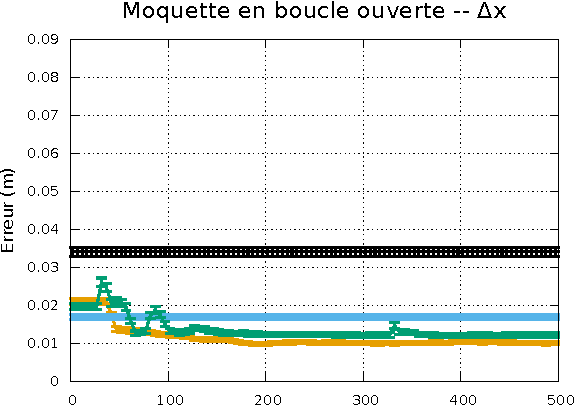
\includegraphics[type=pdf,ext=.pdf,read=.pdf,width=0.2\linewidth]{../plot/OdometryLWPR/carpet_open_convergence_x}
    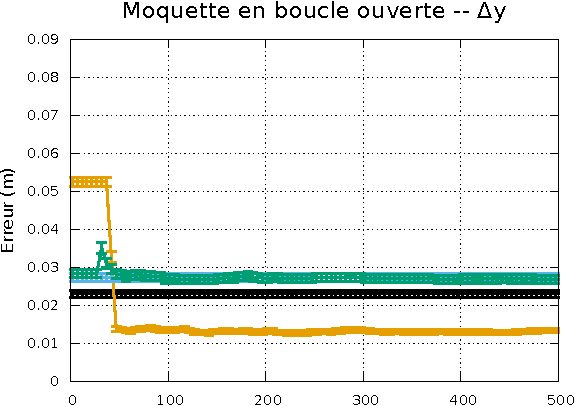
\includegraphics[type=pdf,ext=.pdf,read=.pdf,width=0.2\linewidth]{../plot/OdometryLWPR/carpet_open_convergence_y}
    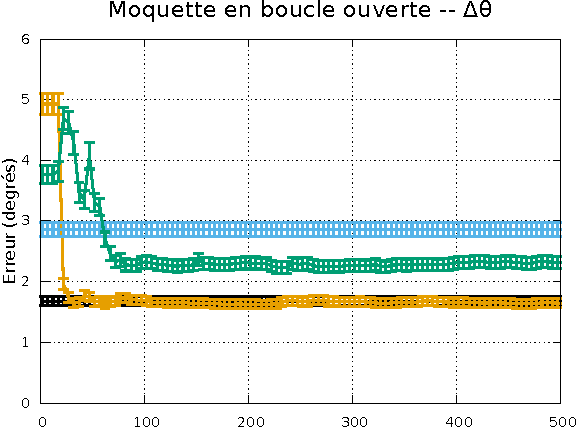
\includegraphics[type=pdf,ext=.pdf,read=.pdf,width=0.2\linewidth]{../plot/OdometryLWPR/carpet_open_convergence_yaw}
    \newline
    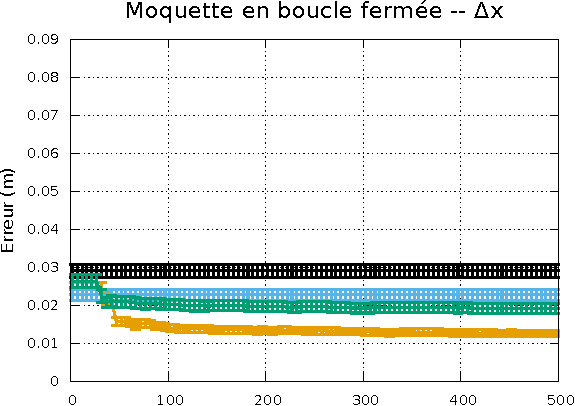
\includegraphics[type=pdf,ext=.pdf,read=.pdf,width=0.2\linewidth]{../plot/OdometryLWPR/carpet_close_convergence_x}
    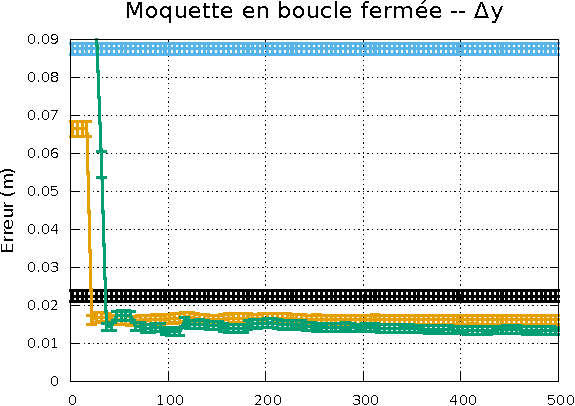
\includegraphics[type=pdf,ext=.pdf,read=.pdf,width=0.2\linewidth]{../plot/OdometryLWPR/carpet_close_convergence_y}
    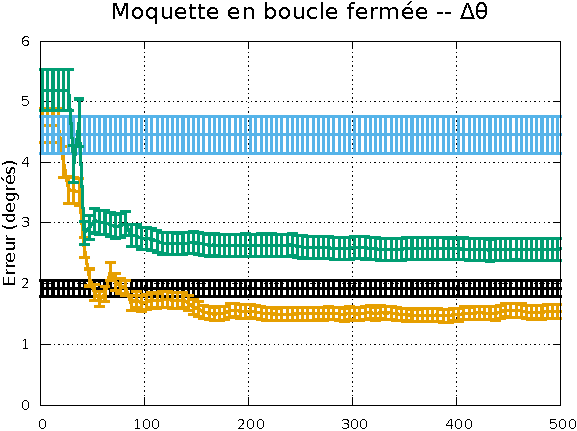
\includegraphics[type=pdf,ext=.pdf,read=.pdf,width=0.2\linewidth]{../plot/OdometryLWPR/carpet_close_convergence_yaw}
    \newline
\end{frame}

\begin{frame}[noframenumbering]{Odométrie et LWPR -- Statistiques}
    \centering
    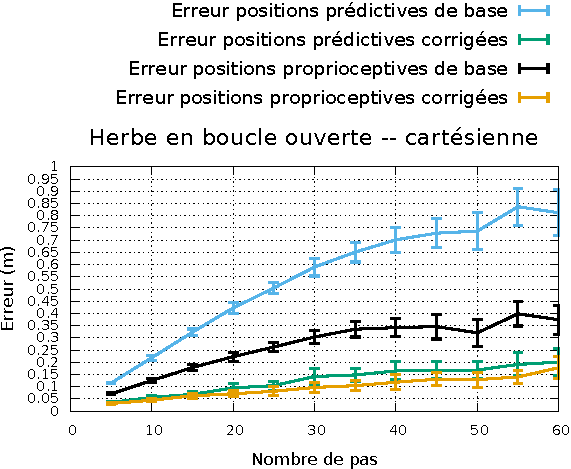
\includegraphics[type=pdf,ext=.pdf,read=.pdf,width=0.25\linewidth]{../plot/OdometryLWPR/grass_open_compare_cart}
    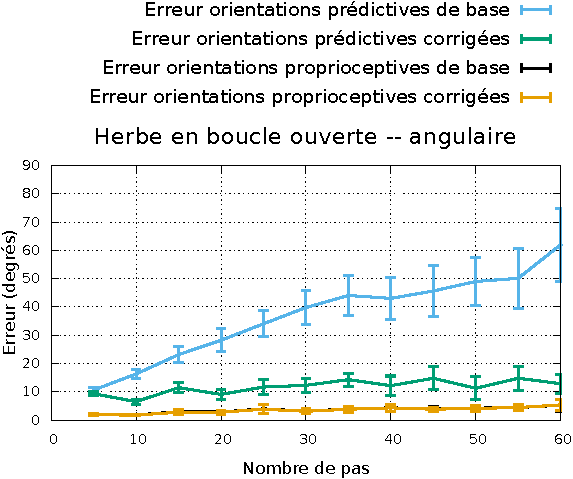
\includegraphics[type=pdf,ext=.pdf,read=.pdf,width=0.25\linewidth]{../plot/OdometryLWPR/grass_open_compare_angle}
    \newline
    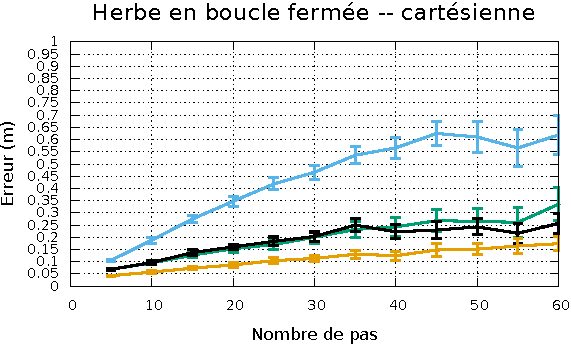
\includegraphics[type=pdf,ext=.pdf,read=.pdf,width=0.25\linewidth]{../plot/OdometryLWPR/grass_close_compare_cart}
    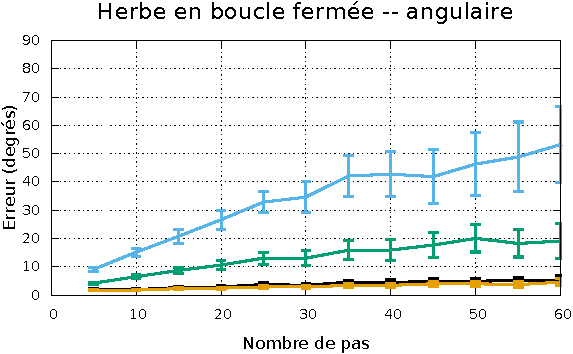
\includegraphics[type=pdf,ext=.pdf,read=.pdf,width=0.25\linewidth]{../plot/OdometryLWPR/grass_close_compare_angle}
    \newline
    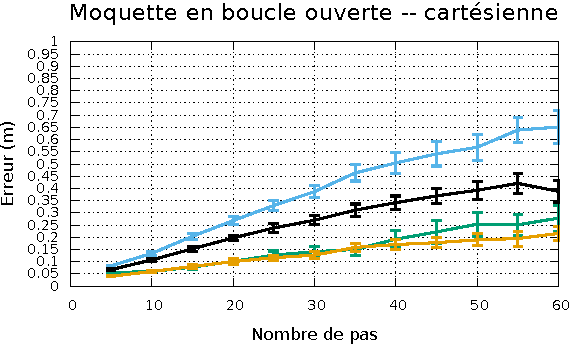
\includegraphics[type=pdf,ext=.pdf,read=.pdf,width=0.25\linewidth]{../plot/OdometryLWPR/carpet_open_compare_cart}
    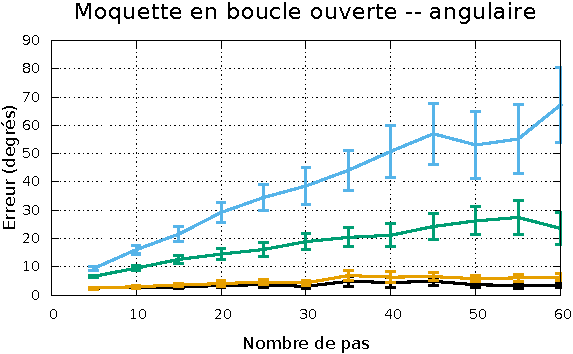
\includegraphics[type=pdf,ext=.pdf,read=.pdf,width=0.25\linewidth]{../plot/OdometryLWPR/carpet_open_compare_angle}
    \newline
    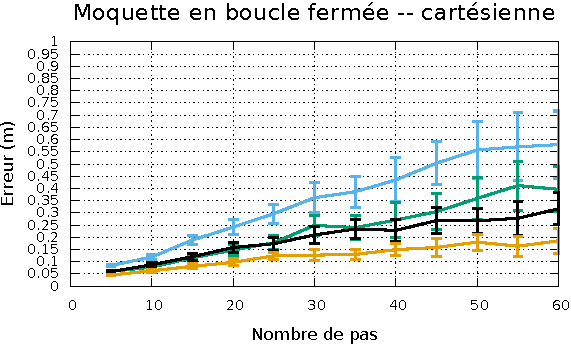
\includegraphics[type=pdf,ext=.pdf,read=.pdf,width=0.25\linewidth]{../plot/OdometryLWPR/carpet_close_compare_cart}
    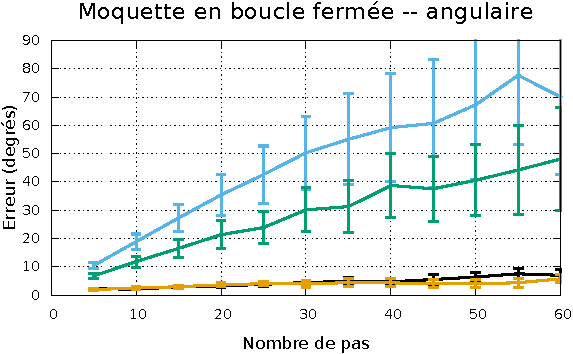
\includegraphics[type=pdf,ext=.pdf,read=.pdf,width=0.25\linewidth]{../plot/OdometryLWPR/carpet_close_compare_angle}
    \newline
\end{frame}

\begin{frame}[noframenumbering]{Odométrie et LWPR -- Trajectoires}
    \centering
    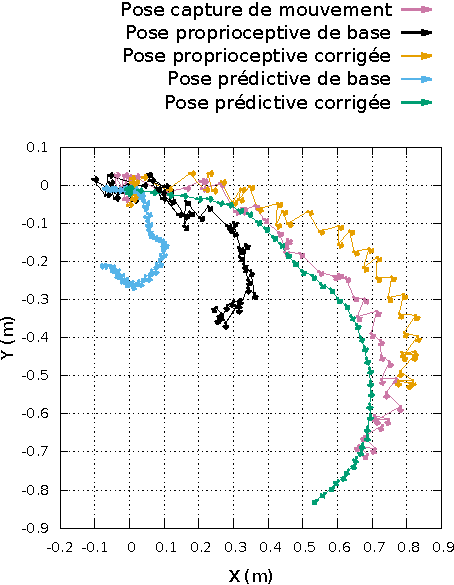
\includegraphics[type=pdf,ext=.pdf,read=.pdf,width=0.3\linewidth]{../plot/OdometryLWPR/grass_open_traj1_pose}
    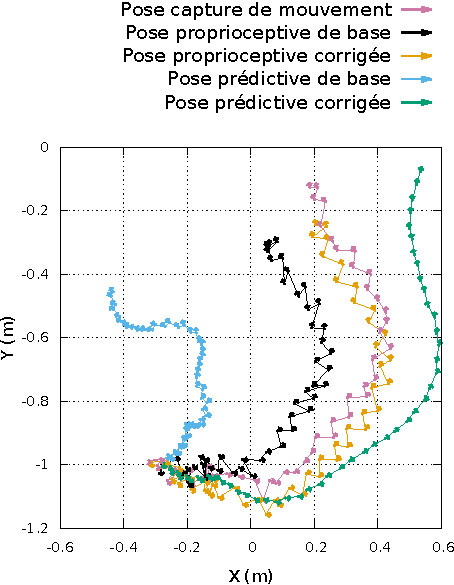
\includegraphics[type=pdf,ext=.pdf,read=.pdf,width=0.3\linewidth]{../plot/OdometryLWPR/grass_open_traj2_pose}
    \newline
    \includegraphics[type=pdf,ext=.pdf,read=.pdf,width=0.3\linewidth]{../plot/OdometryLWPR/grass_open_traj3_pose}
    \includegraphics[type=pdf,ext=.pdf,read=.pdf,width=0.3\linewidth]{../plot/OdometryLWPR/grass_open_traj4_pose}
    \newline
    %\includegraphics[type=pdf,ext=.pdf,read=.pdf,width=0.3\linewidth]{../plot/OdometryLWPR/grass_open_traj5_pose}
    %\includegraphics[type=pdf,ext=.pdf,read=.pdf,width=0.3\linewidth]{../plot/OdometryLWPR/grass_open_traj6_pose}
    %\newline
\end{frame}

\begin{frame}[noframenumbering]{Odométrie et LWPR -- Comparaisons}
    \begin{columns}
        \begin{column}{0.4\linewidth}
            \begin{itemize}
                \item Sans correction, proprioception et prédiction : 
                    stabilisation $\Rightarrow$ réduction de la dérive
                \item Sans correction, prédiction : 
                    herbe $\Rightarrow$ augmentation de la dérive
                \item Avec correction, prédiction : 
                    stabilisation $\Rightarrow$ augmentation la dérive
                \item Avec correction, proprioception et prédiction :
                    herbe $\Rightarrow$ réduction (légère) de la dérive
            \end{itemize}
        \end{column}
        \begin{column}{0.6\linewidth}
            \centering
            \includegraphics[type=pdf,ext=.pdf,read=.pdf,width=0.9\linewidth]{../plot/OdometryLWPR/comparison_values}
        \end{column}
    \end{columns}
\end{frame}

\begin{frame}[noframenumbering]{Odométrie et CMA-ES -- Formules}
    $$
    2
    \begin{bmatrix}
        \text{stepGain} \\
        \text{lateralGain} \\
        \text{turnGain} \\
    \end{bmatrix}
    =
    \begin{bmatrix}
        \Delta x_{\text{base}} \\   
        \Delta y_{\text{base}} \\   
        \Delta \theta_{\text{base}}
    \end{bmatrix}
    =
    \Delta \bm{p}_{\text{base}}
    $$
    $$
    \begin{cases}
    \bm{p}_{0} = \begin{bmatrix} 0 & 0 & 0 \end{bmatrix}^{\mathsf{T}} \\
        \bm{p}_{k+1} = \mathsf{displtInt}\big(\bm{p}_{k}, \mathsf{Correction}_{\Theta}(\Delta \bm{p}_{\text{base}, k}) \big) \\
    \end{cases}
    $$
    $$
    \mathsf{erreurAngulaire} : 
    \big( \theta_{\text{final}}, \theta_{\text{mesure}} \big) 
    \longmapsto 
    \begin{cases}
        \mathsf{angleDistance}(\theta_{\text{final}}, \theta_{\text{mesure}})
        \text{ si } \geqslant \frac{2\pi}{12} \\
        0 \text{ sinon} \\
    \end{cases}
    $$
    \begin{gather*}
    \mathsf{fitness} : 
    \big( \bm{p}_{\text{final}}, \bm{p}_{\text{mesure}} \big)
    =
    \big( \begin{bmatrix} x_{\text{final}}\\ y_{\text{final}}\\ \theta_{\text{final}}\\ \end{bmatrix}, 
    \begin{bmatrix} x_{\text{mesure}}\\ y_{\text{mesure}}\\ \theta_{\text{mesure}}\\ \end{bmatrix} \big)
    \longmapsto \\
    (x_{\text{final}} - x_{\text{mesure}})^{2} + (y_{\text{final}} - y_{\text{mesure}})^{2}
    + \big( \alpha.\mathsf{erreurAngulaire}(\theta_{\text{final}}, \theta_{\text{mesure}}) \big)^{2}
    \end{gather*}
    $$
    \underset{\Theta}{\mathrm{arg~min}} 
    \big( \sqrt{\frac{1}{n}\sum_{i} \mathsf{fitness}(\bm{p}_{\text{final}}^{i, \Theta}, \bm{p}_{\text{mesure}}^{i})} \big)
    $$
\end{frame}

\begin{frame}[noframenumbering]{Odométrie et CMA-ES -- Exploration}
    \centering
    \includegraphics[type=pdf,ext=.pdf,read=.pdf,width=0.65\linewidth]{../plot/OdometryCMAES/walk_orders}
\end{frame}

\begin{frame}[noframenumbering]{Odométrie et CMA-ES -- Paramètres 1}
    \begin{columns}
        \begin{column}{0.5\linewidth}
            \centering
            \includegraphics[type=pdf,ext=.pdf,read=.pdf,width=0.6\linewidth]{../plot/OdometryCMAES/parametersPropOrders}
        \end{column}
        \begin{column}{0.5\linewidth}
            \centering
            \includegraphics[type=pdf,ext=.pdf,read=.pdf,width=0.75\linewidth]{../plot/OdometryCMAES/parametersSimpleOrders}
        \end{column}
    \end{columns}
    \centering
\end{frame}

\begin{frame}[noframenumbering]{Odométrie et CMA-ES -- Paramètres 2}
    \centering
    \includegraphics[type=pdf,ext=.pdf,read=.pdf,height=0.85\textheight]{../plot/OdometryCMAES/parametersFullOrders}
\end{frame}

\begin{frame}[noframenumbering]{Odométrie et CMA-ES -- Trajectoires}
    \centering
    \includegraphics[type=pdf,ext=.pdf,read=.pdf,width=0.20\linewidth]{../plot/OdometryCMAES/ordersTraj1}
    \includegraphics[type=pdf,ext=.pdf,read=.pdf,width=0.20\linewidth]{../plot/OdometryCMAES/ordersTraj2}
    \includegraphics[type=pdf,ext=.pdf,read=.pdf,width=0.20\linewidth]{../plot/OdometryCMAES/ordersTraj3}
    \newline
    \includegraphics[type=pdf,ext=.pdf,read=.pdf,width=0.20\linewidth]{../plot/OdometryCMAES/ordersTraj4}
    \includegraphics[type=pdf,ext=.pdf,read=.pdf,width=0.20\linewidth]{../plot/OdometryCMAES/ordersTraj5}
    \includegraphics[type=pdf,ext=.pdf,read=.pdf,width=0.20\linewidth]{../plot/OdometryCMAES/ordersTraj6}
    \newline
    \includegraphics[type=pdf,ext=.pdf,read=.pdf,width=0.20\linewidth]{../plot/OdometryCMAES/ordersTraj7}
    \includegraphics[type=pdf,ext=.pdf,read=.pdf,width=0.20\linewidth]{../plot/OdometryCMAES/ordersTraj8}
    \includegraphics[type=pdf,ext=.pdf,read=.pdf,width=0.20\linewidth]{../plot/OdometryCMAES/ordersTraj9}
    \newline
\end{frame}

\begin{frame}[noframenumbering]{Politique d'approche de la balle}
    \begin{block}{Problème de l'approche}
        \begin{itemize}
            \item Contrôle de la marche 
            \item $\Rightarrow$ position + orientation de tir
            \item Éviter la collision de la balle
        \end{itemize}
    \end{block}
    \begin{itemize}
        \item Optimisation en simulation
        \item Précompensation des défauts
        \item Modèle du bruit de déplacement
    \end{itemize}
    Politiques comparées :
    \begin{itemize}
        \item Approche experte (machine à états)
        \item Approche experte + optimisation CMA-ES
        \item Politique de contrôle MDP continues
    \end{itemize}
\end{frame}

\begin{frame}[noframenumbering]{Odométrie et CMA-ES -- Comparaisons approches}
    Simulation :\\
    \begin{tabular}{|l|c|c|c|}
        \hline
            & \textit{Expert} & \textit{CMA-ES} & \textit{RFPI} \\
        \hline
        Marche holonome     & 31.84      & 14.90  & 11.88      \\
        Marche quasiment non holonome   & 44.12      & 36.18  & 15.97 \\
        \hline
    \end{tabular}
    \vspace{4em}
    \newline
    Réalité :\\
    \begin{tabular}{|l|c|c|c|}
        \hline
            & \textit{Expert} & \textit{CMA-ES} & \textit{RFPI} \\
        \hline
        Marche holonome   & 19.98      & 13.72  & 11.45      \\
        Marche quasiment non holonome & 48.14      & 25.69  & 18.81 \\
        \hline
    \end{tabular}
\end{frame}

\begin{frame}[noframenumbering]{Odométrie et CMA-ES -- Trajectoires approches}
    \centering
    \includegraphics[type=pdf,ext=.pdf,read=.pdf,width=0.65\linewidth]{../plot/OdometryCMAES/robotTrajs}
\end{frame}

\begin{frame}[noframenumbering]{Tir expert 2016}
    \centering
    \includegraphics[type=pdf,ext=.pdf,read=.pdf,width=1.0\linewidth]{../plot/kickgreg_vel}
\end{frame}

\begin{frame}[noframenumbering]{Modélisation dynamique}
    Équation de la dynamique :
    $$
    \begin{cases}
    \bm{H}\bm{\ddot{q}} + \bm{C} - \bm{K}^\T\bm{\lambda} = \bm{\tau} \\
    \bm{K}\bm{\ddot{q}} = \bm{k}
    \end{cases}
    $$
    Contraintes :
    $$
    \bm{K}\bm{\ddot{q}} = \bm{k}
    $$
    Impulsions :
    $$
    \begin{cases}
        \bm{H}(\bm{\dot{q}}_{+}-\bm{\dot{q}}_{-}) - \bm{K}^\T\bm{\Lambda} = \bm{0} \\
    \bm{K}\bm{\dot{q}}_{+} = \bm{0} \\
    \end{cases}
    $$
    Contacts (LCP) :
    $$
    \dot{\bm{\zeta}} = \bm{M}\bm{\lambda} + \bm{d}
    $$
    $$
    \begin{cases}
    \bm{M} = \bm{K}\bm{H}^{-1}\bm{K}^\T & \in \mathbb{R}^{m \times m}\\
    \bm{d} = \bm{K}\bm{H}^{-1}\left(\bm{\tau} - \bm{C}\right) - \bm{k} & \in \mathbb{R}^{m}\\
    \end{cases}
    $$
\end{frame}

\begin{frame}[noframenumbering]{Modélisation des servomoteurs}
    Modèle électrique (linéaire) :
    $$
    U = \tau_{\text{moteur}} \frac{R}{k_{c}} + \omega k_{e}
    $$
    Réduction :
    $$
    r \omega = \dot{q}
    $$
    Couples :
    $$
    \tau_{\text{externe}} = \frac{1}{r} \tau_{\text{moteur}} - \tau_{\text{friction}} - \tau_{\text{inertie}}
    $$
    Inertie :
    $$
    \tau_{\text{inertie}} = J \ddot{q}
    $$
    Frottement :
    $$
    \mathsf{Friction} :~ \dot{q}
    \longmapsto 
    \tau_{\text{friction}}
    =
    \mu_{\text{vis}} \dot{q} 
    + \big( 
    \mu_{\text{break}} \beta 
    + \mu_{\text{coulomb}} (1-\beta) \big) 
    \eta
    $$
    $$
    \beta = e^{-|\frac{\dot{q}}{\mu_{\text{vel}}}|}
    $$
    $$
    \eta = \mathsf{tanh}(\mu_{\text{reg}}\dot{q})
    $$
\end{frame}

\begin{frame}[noframenumbering]{Polynome quintique}
    \centering
    \includegraphics[type=pdf,ext=.pdf,read=.pdf,width=0.6\linewidth]{../plot/quintic_runge}
\end{frame}

\begin{frame}[noframenumbering]{Correction de mouvement}
    \centering
    \begin{tabular}{|l|l|l|}
        \hline
        Mouvement & Erreur moyenne (degrés) & Erreur maximale (degrés) \\
        \hline
        \multicolumn{3}{|c|}{Dans le simulateur (identifié)} \\
        \hline
        Original & 2.56 & 17.9 \\
        Feedforward & 1.20 & 9.61 \\
        Simulateur & 0.45 & 3.21 \\
        \hline
        \multicolumn{3}{|c|}{Sur le robot Sigmaban} \\
        \hline
        Original & 2.46 & 22.1 \\
        Feedforward & 0.88 & 12.0 \\
        Simulateur & 0.71 & 5.94 \\
        \hline
    \end{tabular}
\end{frame}

\begin{frame}[noframenumbering]{Perspectives -- Mouvements}
    \begin{itemize}
        \setlength\itemsep{1.0em}
        \item Amélioration du simulateur
            \begin{itemize}
                \item Glissement
                \item Dynamique impulsive
            \end{itemize}
        \item Étude du tir expert
        \item Transfert vers la réalité
            \begin{itemize}
                \item Identification dynamique
                \item \customtextcolor{(Hanna et Stone, 2017)} $\Rightarrow$ apprentissage
            \end{itemize}
        \item Étude de la modélisation
            \begin{itemize}
                \item Apport de chaque modèle
            \end{itemize}
    \end{itemize}
\end{frame}

\begin{frame}[noframenumbering]{Architecture logicielle}
    \centering
    \includegraphics[width=1.0\linewidth]{../media/code_graph.png}
\end{frame}

